\documentclass[aspectratio=169]{beamer}

\usepackage[utf8]{inputenc} % mindenképp maradjon az utf-8 kódolás
\usepackage[magyar]{babel}
\usepackage[T1]{fontenc}
\usepackage{amsmath}
\usepackage{amsfonts}
\usepackage{amssymb}
\usepackage{graphics} % grafikus elemek, képek berakásához
\usepackage{blindtext}
%\usepackage{hyperref} % PDF hivatkozásokhoz kell
\usepackage[hang]{caption}
\usepackage{xcolor}
\usepackage{siunitx}
%\usepackage[affil-it]{authblk}

%\definecolor{rosewood}{rgb}{0.6, 0.0, 0.04}
%\definecolor{indigo(dye)}{rgb}{0.0, 0.25, 0.42}

\usetheme{Warsaw}	% téma
\usefonttheme{serif}	% gyönyörű talpas betűtípus

\setbeamercovered{transparent=30}
\beamertemplatenavigationsymbolsempty % a pdf-be ágyazott navigációs gombok kikapcsolása

\title{2,4 GHz-es nyomtattott BIFA tervezése}			% cím
\subtitle{} 	% alcím

\date{\today}

\author{Szilágyi Gábor}	% szerző

\institute{Silicon Laboratories} % intézmény vagy más infó a szerzőről

\begin{document}
\maketitle	% címoldal
\begin{frame}
	\frametitle{Részfeladatok}
			\begin{enumerate}
				\item<0-3> Szimmetrikus tápvonal \\[1.5ex]
				\item<0-3> Szimmetrikus IFA (BIFA) \\[1.5ex]
				\item<0-2> Nyomtatott balun transzformátor \\[1.5ex]
				\item<0-1> Áramblokkoló mintázat
			\end{enumerate}
\end{frame}
\begin{frame}
	\frametitle{Szimmetrikus tápvonal}
	\framesubtitle{CPS -- coplanar strip}
	\centering
	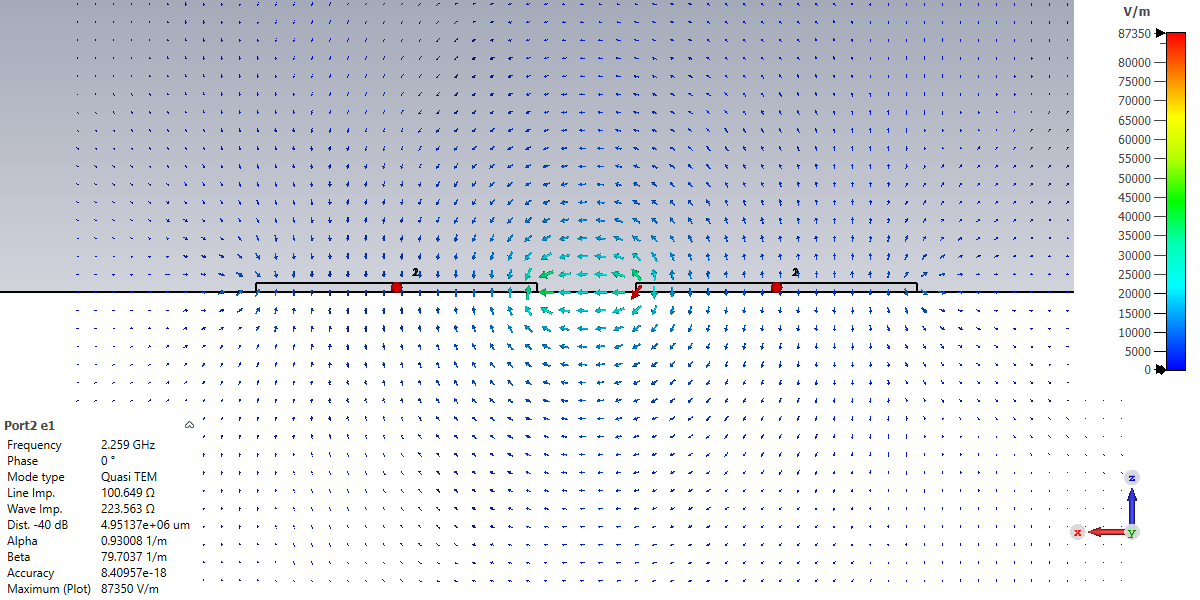
\includegraphics[width=\textwidth]{e1_2.png}
\end{frame}
\begin{frame}
	\frametitle{Antenna}
	\framesubtitle{Alapelv}
	\begin{columns}	
		\column{0.6\textwidth}
			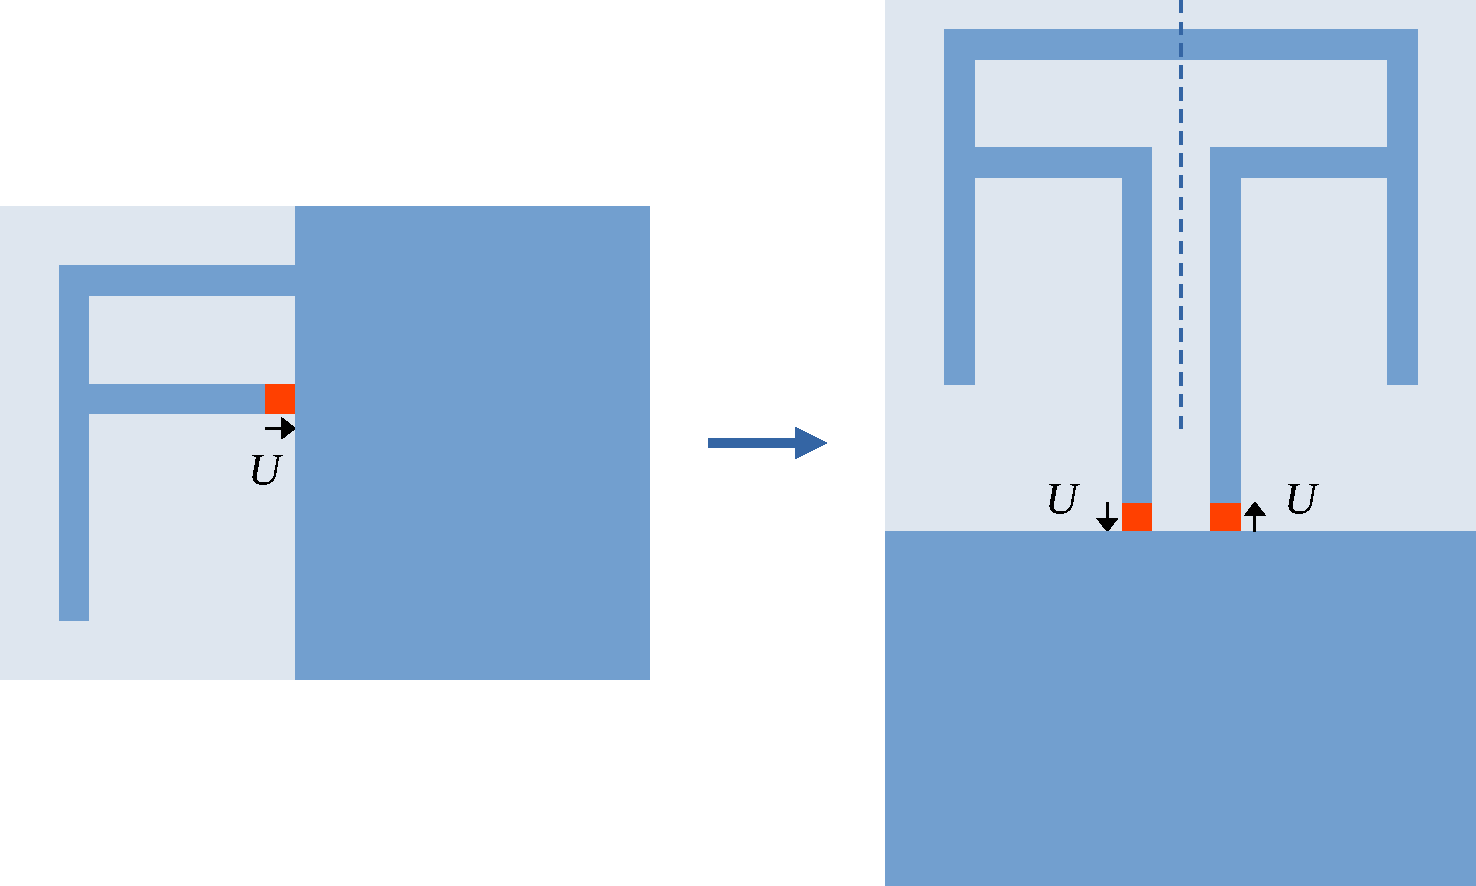
\includegraphics[width=\textwidth]{ifa-bifa.pdf}
		\column{0.38\textwidth}
			Csökken a NYÁK hatása\\[2ex]
			Rezonálhat
	\end{columns}
\end{frame}
\begin{frame}
	\frametitle{Antenna}
	\framesubtitle{Variációk}
		\centering
		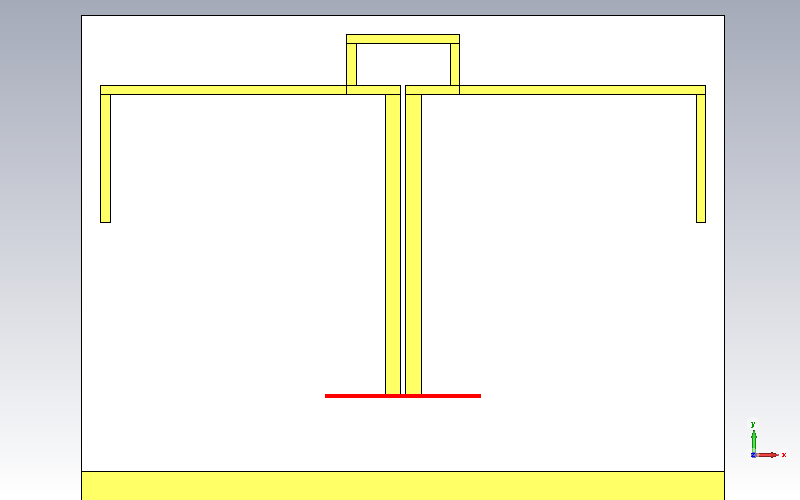
\includegraphics[width=0.38\textwidth]{bifa_3D.png}
		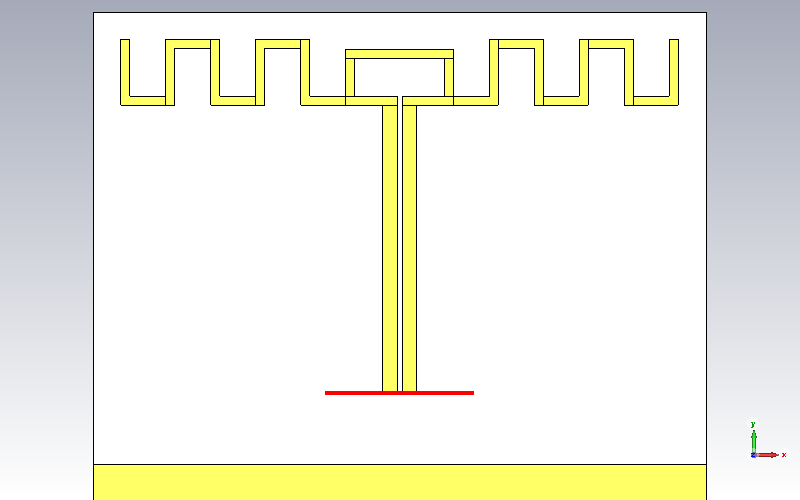
\includegraphics[width=0.38\textwidth]{bifa_meandered_3D.png}
		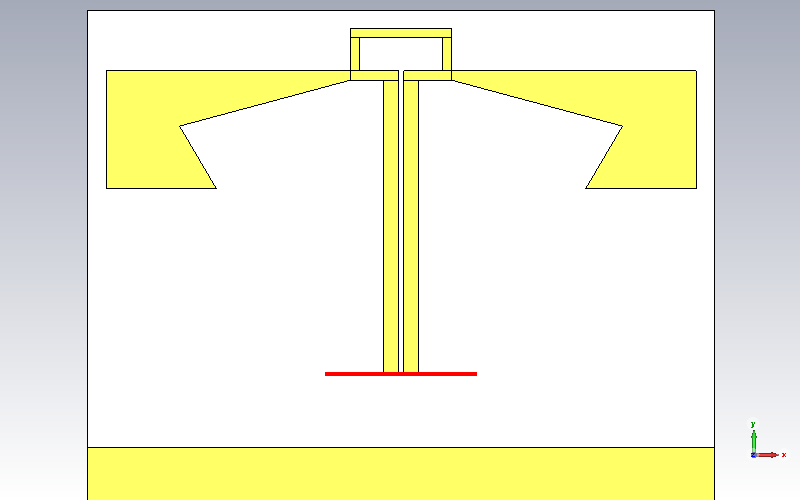
\includegraphics[width=0.38\textwidth]{bifa_broadband_3D.png}
\end{frame}
\begin{frame}
	\frametitle{Antenna}
	\framesubtitle{$Q$}
	\begin{columns}
		\column{0.48\textwidth}
			Közelítések $Q$-ra:\\
			\begin{align*}
				s & = \frac{3}{2}, \quad \sqrt{\beta} = \frac{s-1}{2\sqrt{s}} \\
				Q(\omega) & \simeq \frac{2 \sqrt{\beta}}{\text{FBW}_V(\omega)} \\
				\vspace{\fill}\\
				Q(\omega) & \simeq \frac{\omega}{2 R(\omega)}|Z'(\omega)|
			\end{align*}
		\column{0.48\textwidth}
			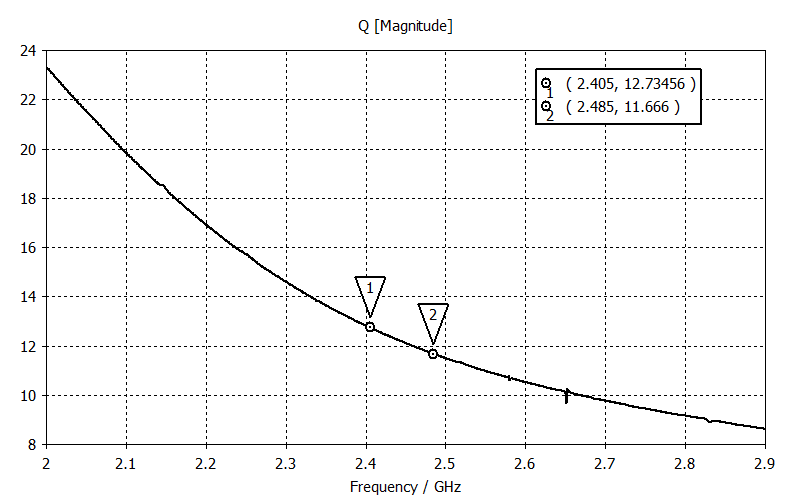
\includegraphics[width=\textwidth]{bifa_broadband_QZ.png}
	\end{columns}
\end{frame}
\begin{frame}
	\frametitle{Antenna}
	\framesubtitle{$S_{11}$}
		\centering
		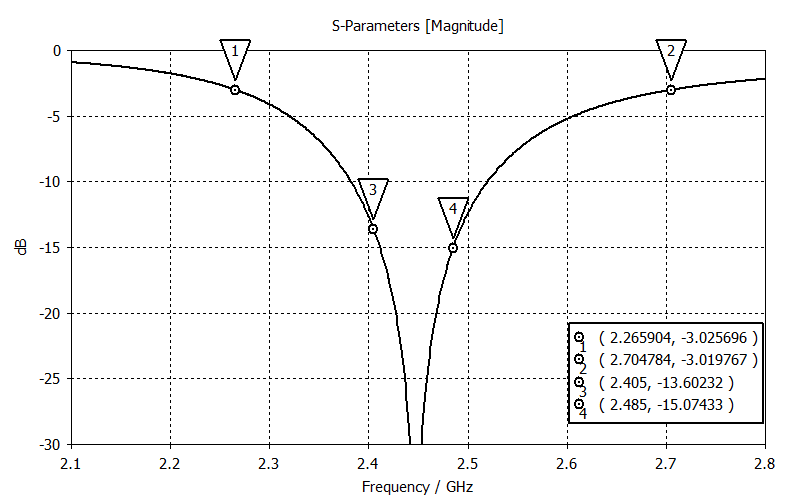
\includegraphics[width=0.8\textwidth]{bifa_broadband_S11_dB.png}
\end{frame}
\begin{frame}
	\frametitle{Antenna}
	\framesubtitle{Iránykarakterisztika}
		\begin{columns}
			\column{0.3\textwidth}
				\centering
				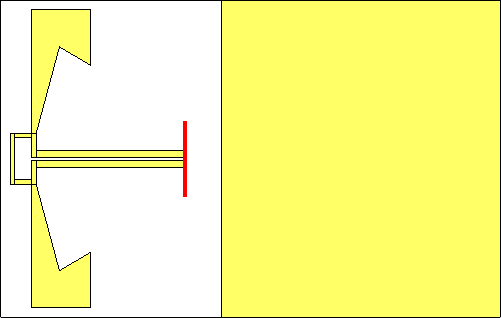
\includegraphics[width=\textwidth]{lying_bifa_bb_3D.png}
			\column{0.68\textwidth}
				\centering
				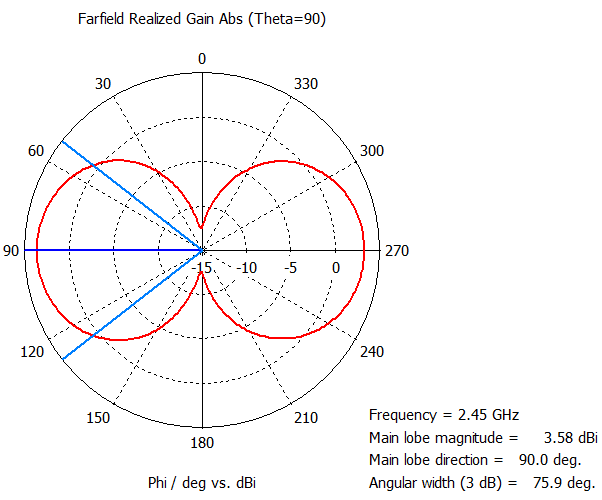
\includegraphics[width=0.8\textwidth]{bifa_broadband_pattern_theta90.png}
		\end{columns}
\end{frame}
\begin{frame}
	\frametitle{Balun transzformátor}
		\centering
		Impedanciatranszformáció: \SI{50}{\ohm} --- \SI{100}{\ohm} \\
		Legjobb $S_{11}$ = -9,2 dB \\
		\vspace{\fill}
		\begin{columns}
			\column{0.1\textwidth}
				\centering
			\column{0.8\textwidth}
				\centering
				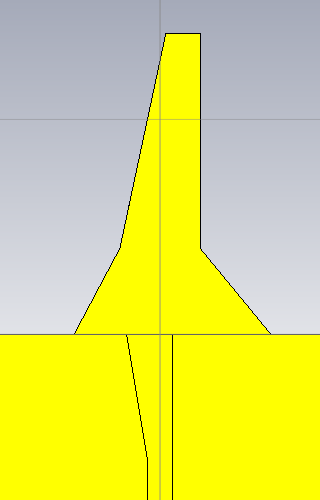
\includegraphics[width=0.3\textwidth]{balun_1.png}
				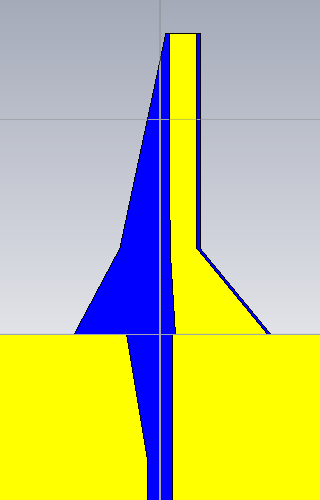
\includegraphics[width=0.3\textwidth]{balun_2.png}
				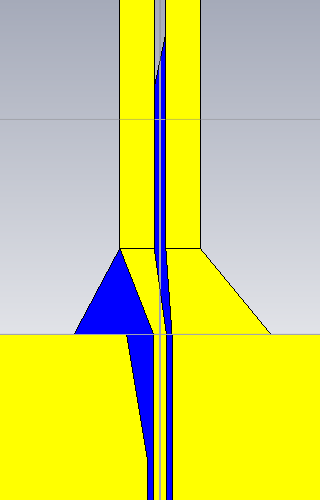
\includegraphics[width=0.3\textwidth]{balun_3.png}
			\column{0.1\textwidth}
				\centering
		\end{columns}
\end{frame}
\begin{frame}
	\centering
		\begin{columns}
		\centering
			\column{0.7\textwidth}
				\centering
				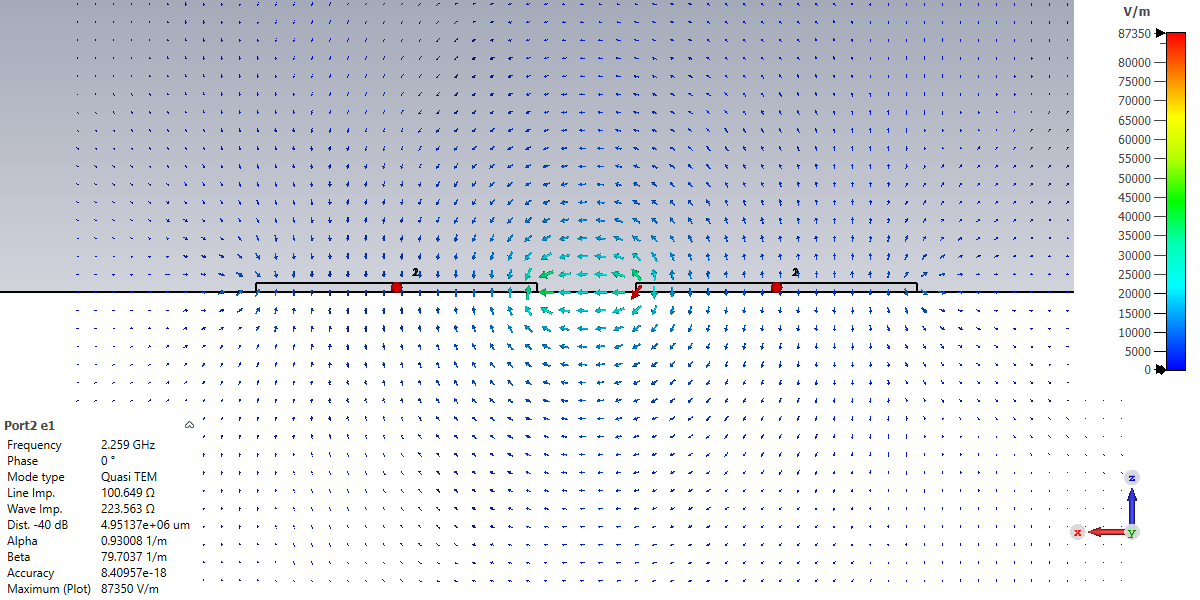
\includegraphics[width=0.45\textwidth]{e1_2.png}
				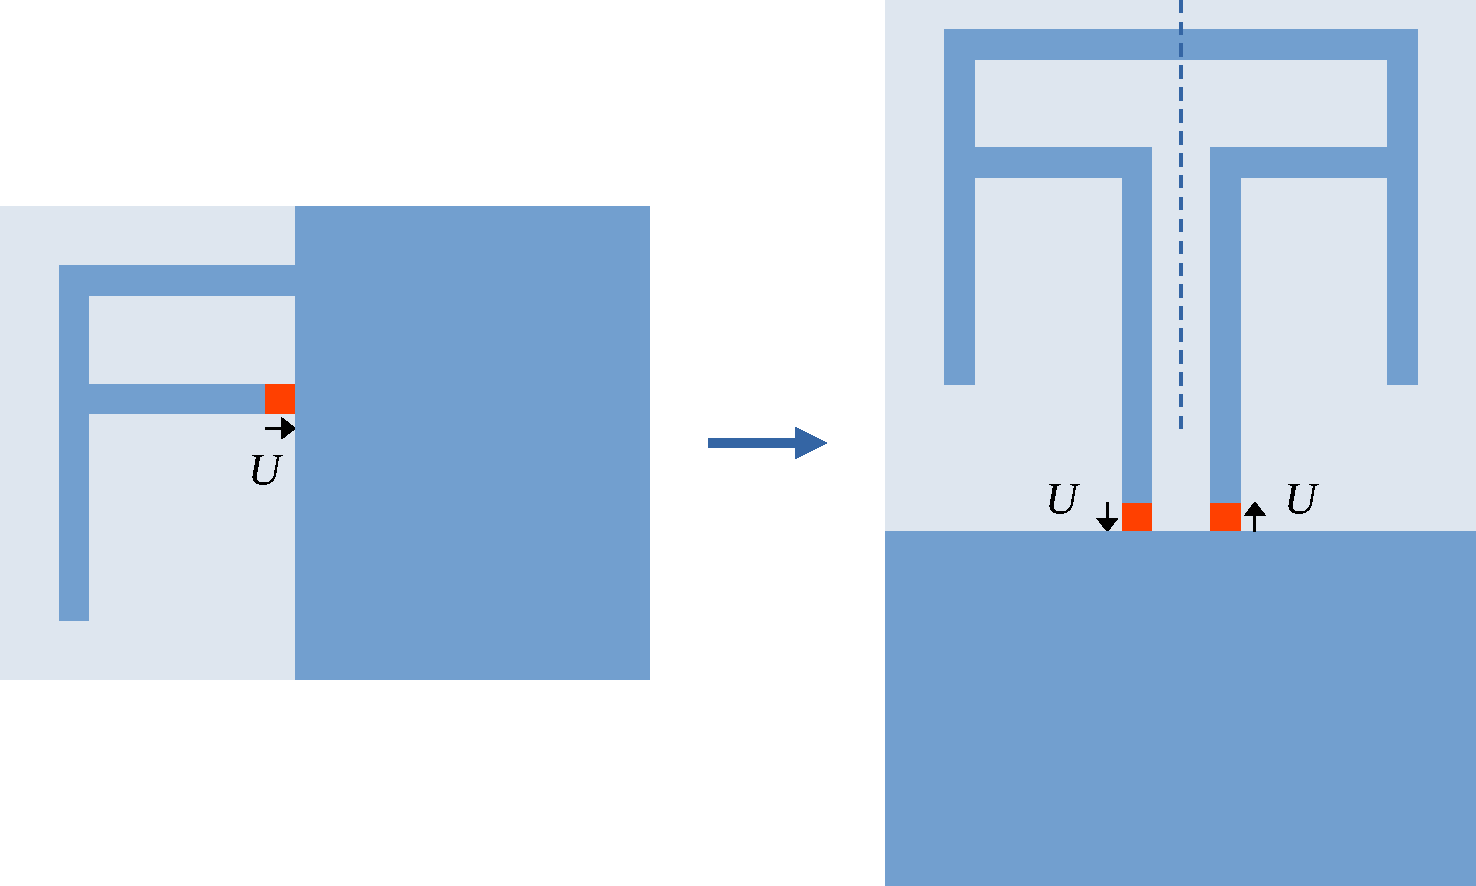
\includegraphics[width=0.45\textwidth]{ifa-bifa.pdf}
				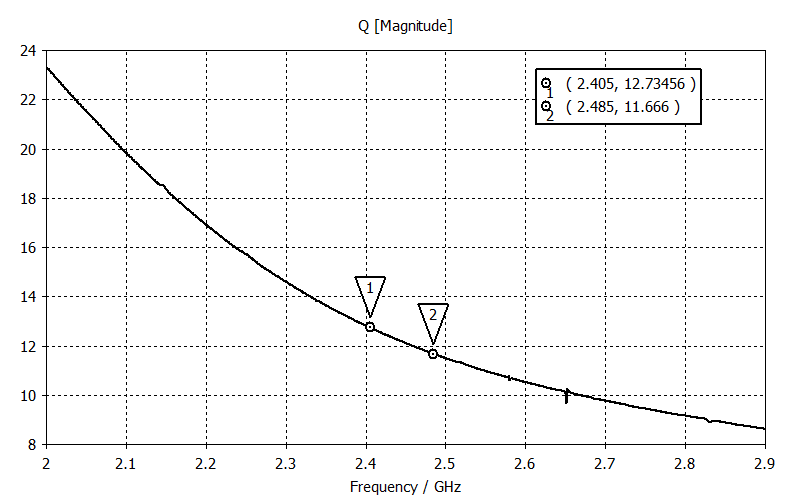
\includegraphics[width=0.3\textwidth]{bifa_broadband_QZ.png}
				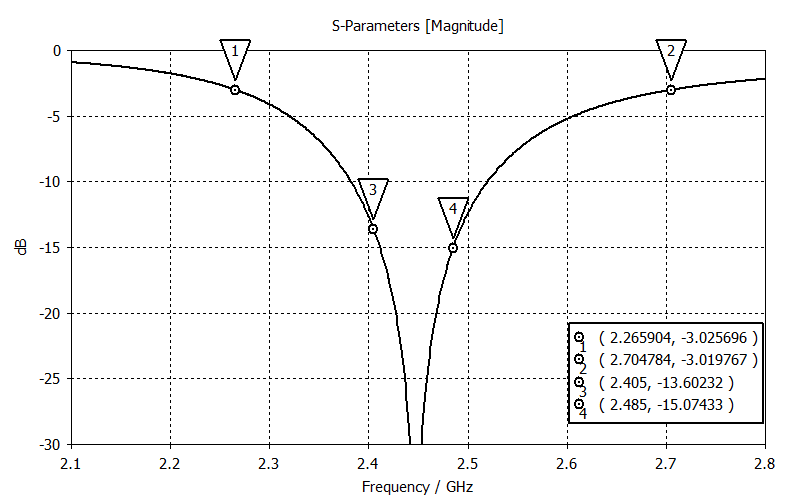
\includegraphics[width=0.3\textwidth]{bifa_broadband_S11_dB.png}
				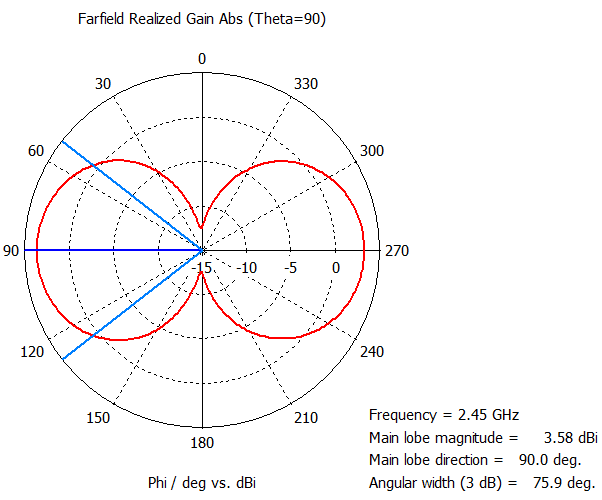
\includegraphics[width=0.3\textwidth]{bifa_broadband_pattern_theta90.png}
			\column{0.3\textwidth}
				\centering
				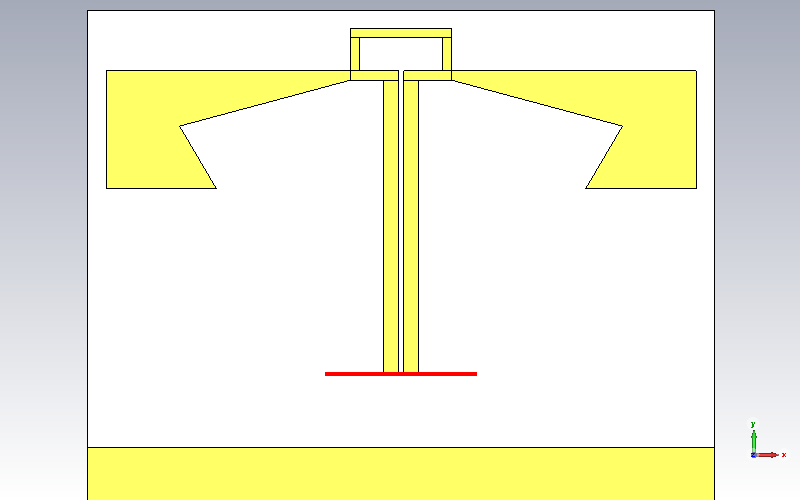
\includegraphics[width=\textwidth]{bifa_broadband_3D.png}\\
				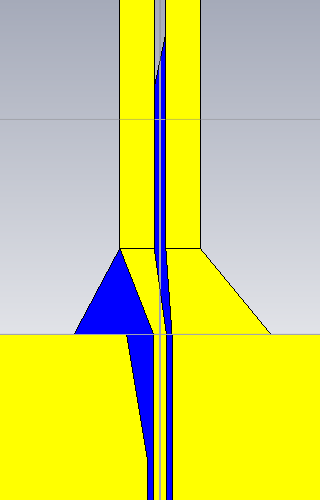
\includegraphics[width=0.7\textwidth]{balun_3.png}
		\end{columns}
\end{frame}
% \begin{frame}
	% \frametitle{Az egydimenziós modell}
	% \begin{columns}
		% \column{0.48\textwidth}
			% A következő egyszerűsítésekkel jutunk 3D-ből az 1D plazmához: \\
			% \begin{itemize}
				% \item A töltetlen $Xe$ részecskéket elhagyjuk
				% \item Az ütközésektől eltekintünk
				% \item Csak az elektronok mozgását vizsgáljuk
				% \item Pontszerű részecskék helyett felületi töltéssűrűséggel rendelkező, az $x$ tengelyre merőleges lapok
				% \item A pozitív töltésű $Xe^+$ ionokat helyhez kötött háttér-töltéssűrűségnek vesszük
			% \end{itemize}
		% \column{0.48\textwidth}
			% \begin{itemize}
				% \item A szimulációs tér egydimenziós és ciklikus, $x=0 \Longleftrightarrow x=N_g$
				% \item A külső elektromos teret 0-nak vesszük
				% \item A mégneses térnek nincs hatása 1D-ben
			% \end{itemize}
	% \end{columns}
% \end{frame}
% \begin{frame}
	% \frametitle{A Particle-Mesh módszer}
	% \begin{columns}
		% \column{0.48\textwidth}
			% Egy kis random szöveg
		% \column{0.48\textwidth}
			% \begin{figure}
				% \includegraphics[draft]{/home/g/Pictures/nap.png}
			% \end{figure}
	% \end{columns}
% \end{frame}
\end{document}